\section{Resultados e Discussão}

\subsection{Sumarização dos resultados}

Foram realizadas \totalExecucoes{} execuções completas, com \totalAvaliacoes{} avaliações de mutantes (excluídos os erros de execução). Por execução, o PIT gerou \gerJavaFracaCem{} mutantes com seu conjunto padrão e o StrykerJS, \gerNodeFracaCem; no recorte harmonizado, os dois conjuntos ficaram quase do mesmo tamanho (\gerhJavaFracaCem{} e \gerhNodeFracaCem), com a mesma distribuição por classe. A Tabela~\ref{tab:resumo} resume cada configuração, e a Figura~\ref{fig:tentativas} mostra o \ms{} em função do número de tentativas.

\begin{table}[!htbp]
\centering
\caption{\textit{Mutation score} (mediana e intervalo interquartil das 30 execuções) com operadores padrão e harmonizados, cobertura de linhas e ramos e mutantes instáveis (M6), por configuração.}
\label{tab:resumo}
\small\setlength{\tabcolsep}{4pt}
\begin{tabular*}{\textwidth}{@{\extracolsep{\fill}}l l r r c r c r@{}}
\toprule
 & & & \multicolumn{2}{c}{\textit{Mutation score} padrão (\%)} & Harmon. & Cobertura (\%) & \\
Ecossistema & Suíte & Tent. & Mediana & IQR & (\%) & linhas / ramos & Instáveis \\
\midrule
Java & fraca & 10 & \msJavaFracaDez & \msqJavaFracaDez & \mshJavaFracaDez & \coblJavaFracaDez{} / \cobrJavaFracaDez & \instJavaFracaDez \\
 &  & 100 & \msJavaFracaCem & \msqJavaFracaCem & \mshJavaFracaCem & \coblJavaFracaCem{} / \cobrJavaFracaCem & \instJavaFracaCem \\
 &  & 1000 & \msJavaFracaMil & \msqJavaFracaMil & \mshJavaFracaMil & \coblJavaFracaMil{} / \cobrJavaFracaMil & \instJavaFracaMil \\
 & forte & 10 & \msJavaForteDez & \msqJavaForteDez & \mshJavaForteDez & \coblJavaForteDez{} / \cobrJavaForteDez & \instJavaForteDez \\
 &  & 100 & \msJavaForteCem & \msqJavaForteCem & \mshJavaForteCem & \coblJavaForteCem{} / \cobrJavaForteCem & \instJavaForteCem \\
 &  & 1000 & \msJavaForteMil & \msqJavaForteMil & \mshJavaForteMil & \coblJavaForteMil{} / \cobrJavaForteMil & \instJavaForteMil \\
\midrule
Node.js & fraca & 10 & \msNodeFracaDez & \msqNodeFracaDez & \mshNodeFracaDez & \coblNodeFracaDez{} / \cobrNodeFracaDez & \instNodeFracaDez \\
 &  & 100 & \msNodeFracaCem & \msqNodeFracaCem & \mshNodeFracaCem & \coblNodeFracaCem{} / \cobrNodeFracaCem & \instNodeFracaCem \\
 &  & 1000 & \msNodeFracaMil & \msqNodeFracaMil & \mshNodeFracaMil & \coblNodeFracaMil{} / \cobrNodeFracaMil & \instNodeFracaMil \\
 & forte & 10 & \msNodeForteDez & \msqNodeForteDez & \mshNodeForteDez & \coblNodeForteDez{} / \cobrNodeForteDez & \instNodeForteDez \\
 &  & 100 & \msNodeForteCem & \msqNodeForteCem & \mshNodeForteCem & \coblNodeForteCem{} / \cobrNodeForteCem & \instNodeForteCem \\
 &  & 1000 & \msNodeForteMil & \msqNodeForteMil & \mshNodeForteMil & \coblNodeForteMil{} / \cobrNodeForteMil & \instNodeForteMil \\
\midrule
Java & \multicolumn{2}{l}{11 exemplos} & \baseJava & --- & \basehJava & --- & --- \\
Node.js & \multicolumn{2}{l}{11 exemplos} & \baseNode & --- & \basehNode & --- & --- \\
\bottomrule
\end{tabular*}
\end{table}

\begin{figure}[!htbp]
\centering
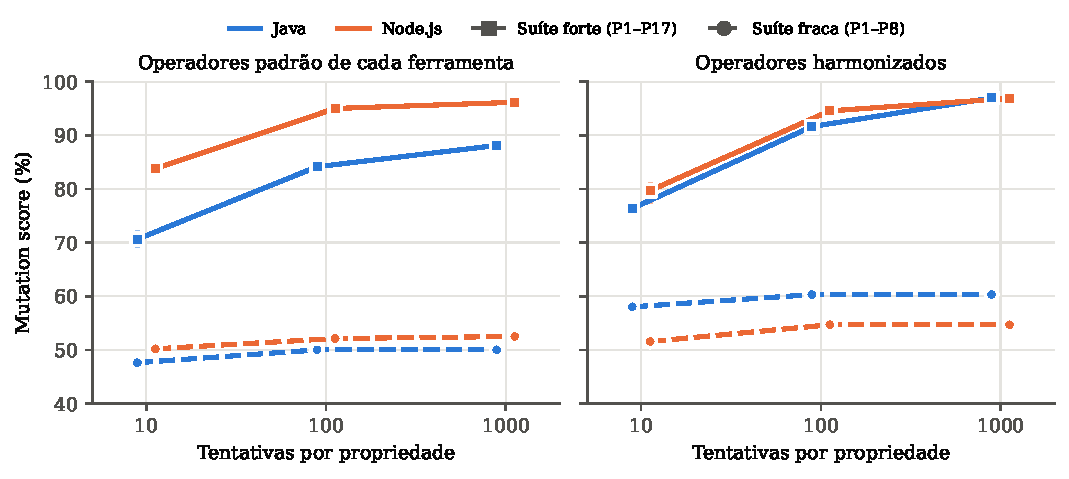
\includegraphics[width=\textwidth]{figuras/fig5_1_score_tentativas.pdf}
\caption{\textit{Mutation score} por número de tentativas, suíte e ecossistema: mediana (marcador) e intervalo interquartil (barra vertical) das 30 execuções. Linhas cheias: suíte forte; tracejadas: suíte fraca.}
\label{fig:tentativas}
\end{figure}

A configuração da versão anterior deste trabalho (suíte fraca, 100 tentativas) foi reproduzida: \msJavaFracaCem\% no Java e \msNodeFracaCem\% no Node.js. As figuras complementares (por classe de mutação, por módulo, por propriedade e de tempo) estão no Apêndice~\ref{ap:figuras}.

\subsection{Discussão dos resultados}

\textbf{QP1 -- Quais regras puderam ser expressas como propriedades equivalentes, e com que oráculo?} Todas. As 17 propriedades foram implementadas nos dois ecossistemas com o mesmo enunciado, as mesmas faixas de geração e o mesmo número de tentativas (M2 = 17/17). A suíte fraca verifica 10 das 20 regras (M1 = 50\%) e nenhuma de suas propriedades confere o valor do preço; a suíte forte verifica as 20 (M1 = 100\%). O tamanho foi equivalente: 336 linhas no Java e 293 no Node.js para a suíte fraca, mais 513 e 446 para as propriedades novas. O jqwik exigiu tipos explícitos para cada dado gerado, enquanto o fast-check compõe geradores em linha; nenhuma propriedade precisou ser adaptada.

\textbf{QP2 -- Qual o \ms{} de cada suíte, e quanto a força do oráculo o altera?} Com 100 tentativas, a suíte fraca detectou \msJavaFracaCem\% (Java) e \msNodeFracaCem\% (Node.js) dos mutantes, e a suíte forte, \msJavaForteCem\% e \msNodeForteCem\%. A suíte forte foi superior em todas as comparações entre execuções ($\hat{A}_{12} = 1$, $p < 0{,}001$ em todas as combinações), com ganho de 23 a 44 pontos. Os 11 cenários de exemplo detectaram \baseJava\% e \baseNode\%, muito acima da suíte fraca, porque conferem valores exatos, inclusive o objeto devolvido por cada operação. Quando as propriedades também conferem valores exatos, elas alcançam os exemplos: no recorte harmonizado, a suíte forte com 1000 tentativas chegou a \mshJavaForteMil\% e \mshNodeForteMil\%, contra \basehJava\% e \basehNode\% dos exemplos.

\textbf{QP3 -- O número de tentativas altera o \ms{}?} Só com propriedades fortes. Na suíte forte, ir de 10 para 100 tentativas elevou o \ms{} de \msJavaForteDez\% para \msJavaForteCem\% no Java e de \msNodeForteDez\% para \msNodeForteCem\% no Node.js; de 100 para 1000, o ganho foi menor (\msJavaForteMil\% e \msNodeForteMil\%). Na suíte fraca, a variação ficou abaixo de 3 pontos, e no Java as 60 execuções com 100 e 1000 tentativas deram o mesmo resultado. Os mutantes que dependem de um valor exato de limite alternam entre detectados e sobreviventes quando há poucas tentativas: na suíte forte, \instJavaForteDez{} (Java) e \instNodeForteDez{} (Node.js) mudaram de resultado entre execuções com 10 tentativas, contra \instJavaForteMil{} e \instNodeForteMil{} com 1000. Mais entradas só ajudam quando o oráculo reconhece o defeito que elas revelam, o que complementa a observação de \citet{ravi2025pbt} de que a maioria das mutações aparece nas primeiras entradas.

\textbf{QP4 -- O \ms{} difere entre os ecossistemas?} Depende dos operadores (Tabela~\ref{tab:testes}). Com os operadores padrão, $H_0$ foi rejeitada em todas as configurações, sempre com o Node.js acima ($\hat{A}_{12} \le 0{,}01$). A diferença vem da ferramenta: o PIT gera mutantes de valor de retorno (por exemplo, devolver \texttt{null} no lugar da reserva atualizada) que as propriedades não observam, porque consultam o estado depois da operação, e o StrykerJS não tem esse operador. No recorte harmonizado, a relação se inverte na suíte fraca (\mshJavaFracaCem\% no Java contra \mshNodeFracaCem\% no Node.js) e, na suíte forte com 1000 tentativas, $H_0$ não foi rejeitada (\mshJavaForteMil\% nos dois, \pEcoForteMilHarm). Com o mutante distinto como unidade e 100 tentativas, nenhuma diferença harmonizada foi significativa (suíte fraca: $\chi^2 = $ \chiFraca, \pchiFraca; forte: $\chi^2 = $ \chiForte, \pchiForte). A inversão na suíte fraca tem uma causa concreta: as duas ferramentas geram o mesmo número de mutantes de condição forçada por regra, mas, numa validação composta como ``nome nulo ou vazio ou capacidade $\le 0$'', o PIT gera pares simétricos (metade força o erro, metade desliga a verificação), enquanto o StrykerJS gera uma versão que força o erro e cinco que desligam partes da verificação. A suíte fraca nunca envia dados inválidos e só percebe as versões que forçam o erro. Isso confirma, para o par PIT/StrykerJS, o que \citet{kintis2018tools} e \citet{monteiro2022tools} observaram entre ferramentas Java: o conjunto de operadores muda o \ms{} mais do que a suíte avaliada.

\begin{table}[!htbp]
\centering
\caption{Teste de $H_0$ (Mann-Whitney U bilateral, $n = 30$ por grupo, $p$ corrigido por Holm) e $\hat{A}_{12}$, a probabilidade de uma execução Java superar uma Node.js. Os testes dos efeitos de suíte, tentativas e tempo estão no Apêndice~\ref{ap:testes}.}
\label{tab:testes}
\small
\begin{tabular*}{\textwidth}{@{\extracolsep{\fill}}l r r r l r r l@{}}
\toprule
 & & \multicolumn{3}{c}{Operadores padrão} & \multicolumn{3}{c}{Operadores harmonizados} \\
Suíte & Tent. & $p$ & $\hat{A}_{12}$ & $H_0$ & $p$ & $\hat{A}_{12}$ & $H_0$ \\
\midrule
Fraca & 10 & \pEcoFracaDez & \aumEcoFracaDez & \decEcoFracaDez & \pEcoFracaDezHarm & \aumEcoFracaDezHarm & \decEcoFracaDezHarm \\
 & 100 & \pEcoFracaCem & \aumEcoFracaCem & \decEcoFracaCem & \pEcoFracaCemHarm & \aumEcoFracaCemHarm & \decEcoFracaCemHarm \\
 & 1000 & \pEcoFracaMil & \aumEcoFracaMil & \decEcoFracaMil & \pEcoFracaMilHarm & \aumEcoFracaMilHarm & \decEcoFracaMilHarm \\
Forte & 10 & \pEcoForteDez & \aumEcoForteDez & \decEcoForteDez & \pEcoForteDezHarm & \aumEcoForteDezHarm & \decEcoForteDezHarm \\
 & 100 & \pEcoForteCem & \aumEcoForteCem & \decEcoForteCem & \pEcoForteCemHarm & \aumEcoForteCemHarm & \decEcoForteCemHarm \\
 & 1000 & \pEcoForteMil & \aumEcoForteMil & \decEcoForteMil & \pEcoForteMilHarm & \aumEcoForteMilHarm & \decEcoForteMilHarm \\
\bottomrule
\end{tabular*}
\end{table}

\textbf{QP5 -- Os mutantes cobertos são também detectados?} Não, quando as propriedades são fracas. Com 100 tentativas, a suíte fraca cobriu \coblJavaFracaCem\% das linhas do domínio no Java e \coblNodeFracaCem\% no Node.js, mas detectou cerca de metade dos mutantes; no módulo de lotes do Java, todos os mutantes foram cobertos e um terço foi detectado (Figura~\ref{fig:cobertura}). Com a suíte forte, a cobertura subiu pouco (\coblJavaForteCem\% e \coblNodeForteCem\%), mas o \ms{} subiu mais de 30 pontos. É a ``lacuna de oráculo'' descrita por \citet{jain2023gap}: a cobertura mostrou onde a suíte não chegava, mas não que metade do código coberto não era verificado.

\textbf{QP6 -- Onde se concentram os mutantes não detectados, e por quê?} A Tabela~\ref{tab:sobreviventes} classifica os mutantes não detectados em ao menos uma execução. Na suíte fraca predominam as \textbf{regras sem propriedade} (\clsJavaFracaRegraPct\% no Java e \clsNodeFracaRegraPct\% no Node.js), principalmente validações de cadastro, evento inativo e entidade inexistente, seguidas dos \textbf{oráculos fracos}. O caso mais claro é o preço: um mutante que faz o subtotal valer sempre zero sobrevive a P1--P4, porque zero é não negativo, um desconto zero está entre zero e o subtotal, a ordem dos itens não muda zero e um cupom inválido não altera zero. Na suíte forte, as regras sem propriedade desaparecem e predominam os mutantes de \textbf{entrada não gerada} (\clsJavaForteEntradaPct\% e \clsNodeForteEntradaPct\%), limites exatos que respondem ao número de tentativas; os oráculos fracos restantes são, no Java, valores de retorno não observados. Os \textbf{equivalentes} são poucos. O oráculo de preço (P9) foi a propriedade que mais matou nos dois ecossistemas, e as propriedades de limite da suíte fraca (P1, P2, P5) não têm nenhuma morte exclusiva na suíte forte (Figura~\ref{fig:propriedades}).

\begin{table}[!htbp]
\centering
\caption{Mutantes não detectados em ao menos uma das 90 execuções de cada combinação de ecossistema e suíte, por classe (todos os operadores avaliados).}
\label{tab:sobreviventes}
\small
\begin{tabularx}{\textwidth}{@{}l Y r r r r@{}}
\toprule
Classe & Principais causas & \multicolumn{2}{c}{Suíte fraca} & \multicolumn{2}{c}{Suíte forte} \\
 & & Java & Node.js & Java & Node.js \\
\midrule
Regra sem propriedade & Validações; evento inativo; entidade inexistente & \clsJavaFracaRegra & \clsNodeFracaRegra & \clsJavaForteRegra & \clsNodeForteRegra \\
Oráculo fraco & Preço verificado só por limites; retornos não observados & \clsJavaFracaOraculo & \clsNodeFracaOraculo & \clsJavaForteOraculo & \clsNodeForteOraculo \\
Entrada não gerada & Limites exatos (validade, mínimo, faixas) & \clsJavaFracaEntrada & \clsNodeFracaEntrada & \clsJavaForteEntrada & \clsNodeForteEntrada \\
Equivalente & Identificadores com outro formato; atalho para cupom nulo & \clsJavaFracaEquivalente & \clsNodeFracaEquivalente & \clsJavaForteEquivalente & \clsNodeForteEquivalente \\
\midrule
Total & & \clsJavaFracaTotal & \clsNodeFracaTotal & \clsJavaForteTotal & \clsNodeForteTotal \\
\bottomrule
\end{tabularx}
\end{table}

\textbf{QP7 -- Qual ecossistema exige mais tempo e mais configuração?} O custo dependeu da suíte (Figura~\ref{fig:tempo}). Com a suíte fraca, o StrykerJS foi mais rápido por mutante (\tpmNodeFracaCem{}~s contra \tpmJavaFracaCem{}~s com 100 tentativas); com a suíte forte, o PIT foi mais rápido no total e por mutante em todos os níveis (\tmutJavaForteMil{}~s contra \tmutNodeForteMil{}~s com 1000 tentativas). A configuração tem tamanho parecido: no Java, dois arquivos e quatro artefatos declarados (jqwik, PIT, o \textit{plugin} JUnit~5 do PIT e JaCoCo); no Node.js, quatro arquivos e quatro pacotes. Dois detalhes do Java não são óbvios: sem o \textit{plugin} JUnit~5 o PIT não encontra os testes, e o reaproveitamento de sementes do jqwik precisa ser desligado para que um mutante não influencie o seguinte.
